L'interfaccia utente proposta presenta tre pannelli:
\begin{itemize}
\item la prima maschera offre semplici funzionalit� per riempire il magazzino simulando l'acquisto di un set. E' prevista la possibilit� di acquistare un set gi� esistente o uno nuovo con pezzi gi� presenti in magazzino. In questo caso si devono aggiornare le quantit� in magazzino con delle \texttt{UPDATE} e non delle \texttt{INSERT}. E' possibile anche visualizzare un semplice grafico a torta per avere un'indicazione di quanti pezzi ci sono in magazzino per costruire un determinato set
\item il secondo pannello offre la possibilit� di scegliere alcuni set e capire quali di questi possono essere costruiti con i pezzi in magazzino. Si ipotizza anche che l'utente possa decidere di accontentarsi di costruire parzialmente i set perch� poi acquister� i pezzi mancati singolarmente. Quindi � possibile impostare una percentuale di completamento.
\item l'ultima maschera infine dovr� elencare i pezzi mancanti  in magazzino per costruire totalmente o in parte un insieme di set e se interessa, cosa conviene acquistare per coprire le mancanze del magazzino.
\end{itemize}

\newpage

\section {Gestione magazzino}

\subsection {Caricamento di un set in magazzino}

\begin{figure}[htbp]
\centering
    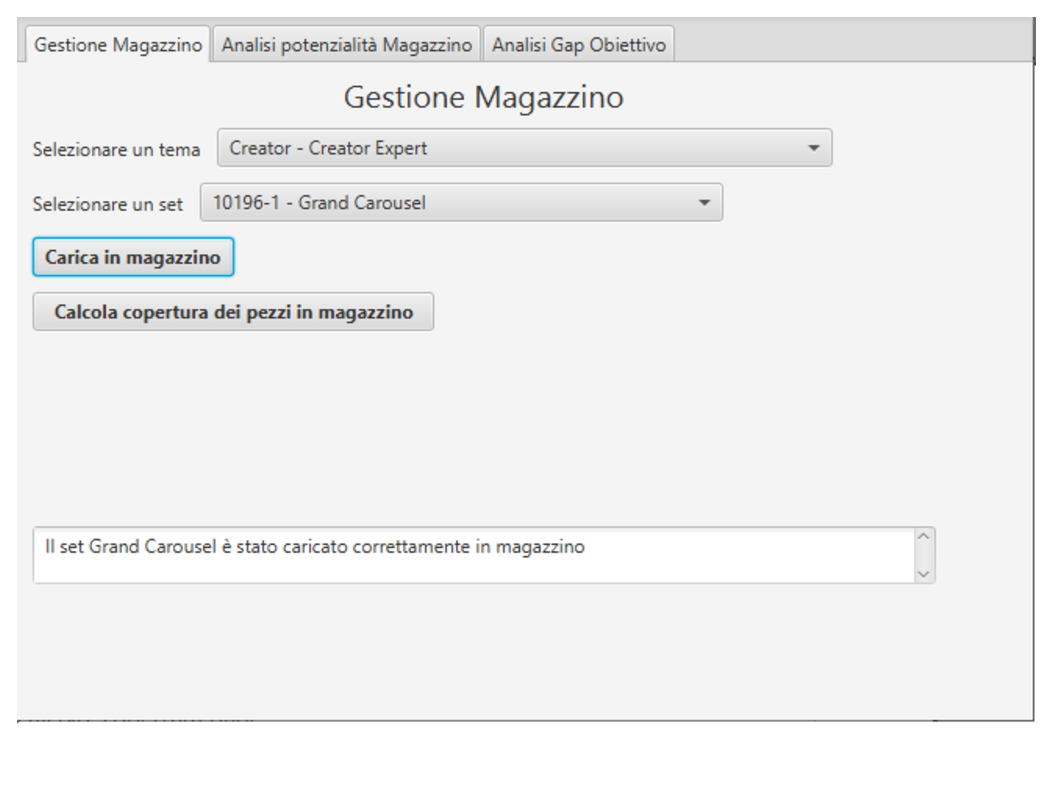
\includegraphics[scale=0.6]{interfaccia_grafica/caricamento_set_magazzino.eps}
\end{figure}


\subsection {Indicazione di quanto manca in magazzino per costruire un set}

\begin{figure}[htbp]
\centering
    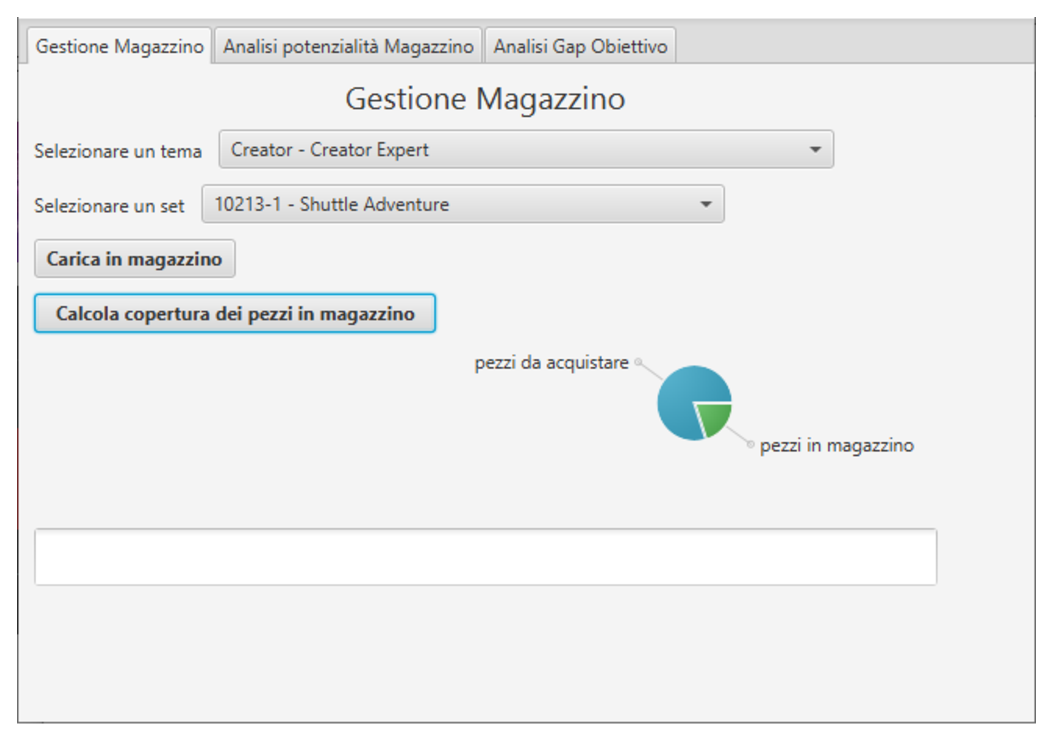
\includegraphics[scale=0.6]{interfaccia_grafica/calcolo_copertura.eps}
\end{figure}

\newpage


\section {Analisi potenzialit� del magazzino}

\begin{figure}[htbp]
\centering
    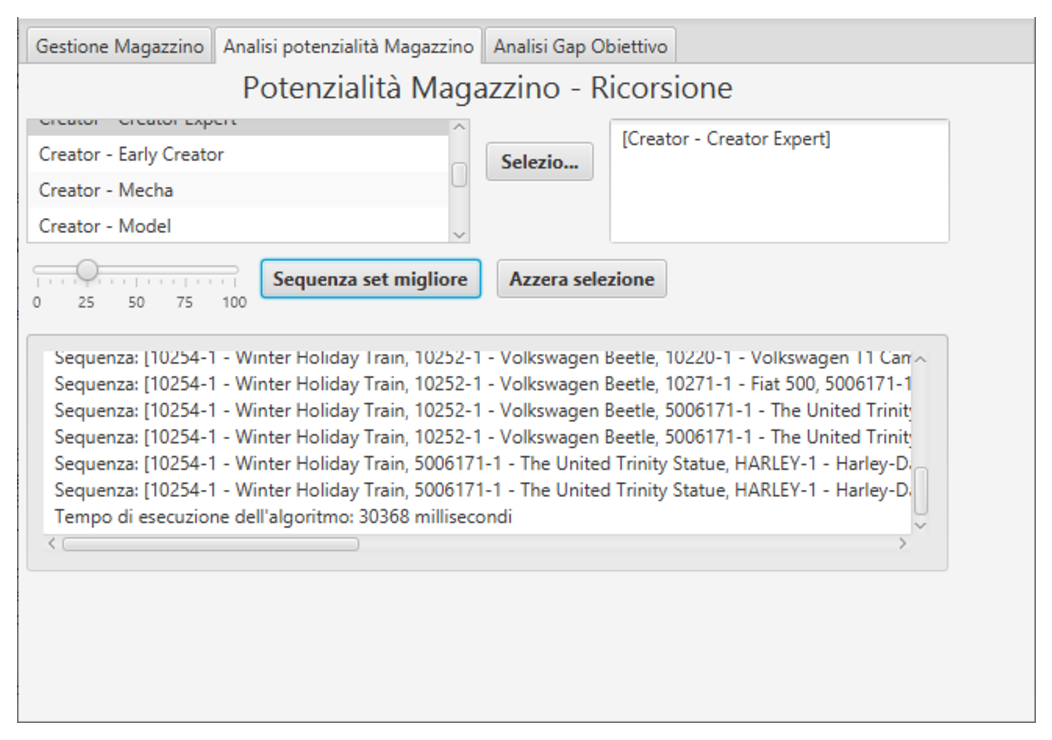
\includegraphics[scale=0.6]{interfaccia_grafica/ricorsione.eps}
\end{figure}

\section {Valutazioni per acquisti futuri}

\subsection {Creazione grafo e albero con set di interesse}

\begin{figure}[htbp]
\centering
    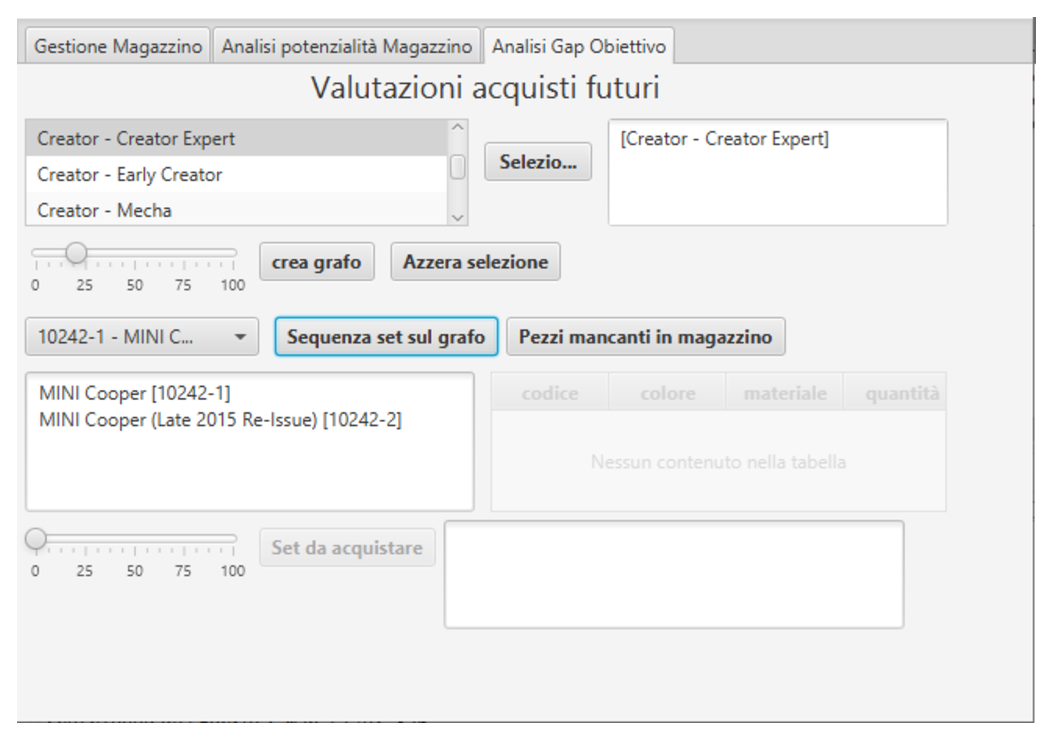
\includegraphics[scale=0.6]{interfaccia_grafica/creazione_grafo.eps}
\end{figure}

\newpage


\subsection {Pezzi mancanti in magazzino}

\begin{figure}[htbp]
\centering
    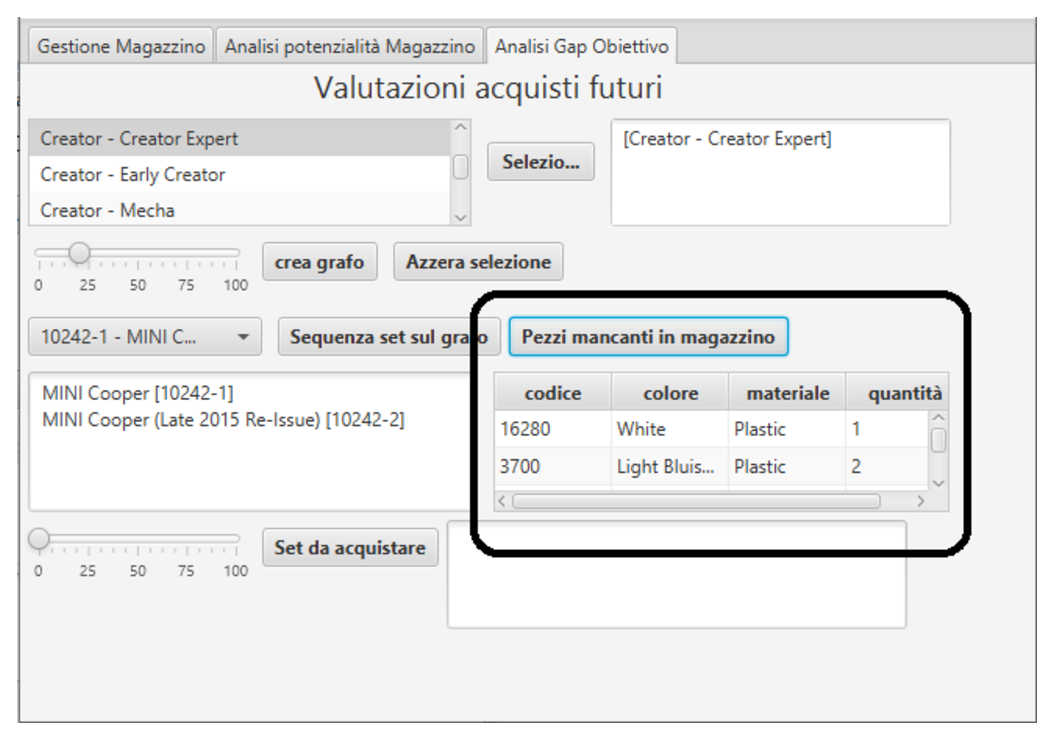
\includegraphics[scale=0.6]{interfaccia_grafica/parti_mancanti.eps}
\end{figure}

\subsection {Cosa conviene acquistare}

\begin{figure}[htbp]
\centering
    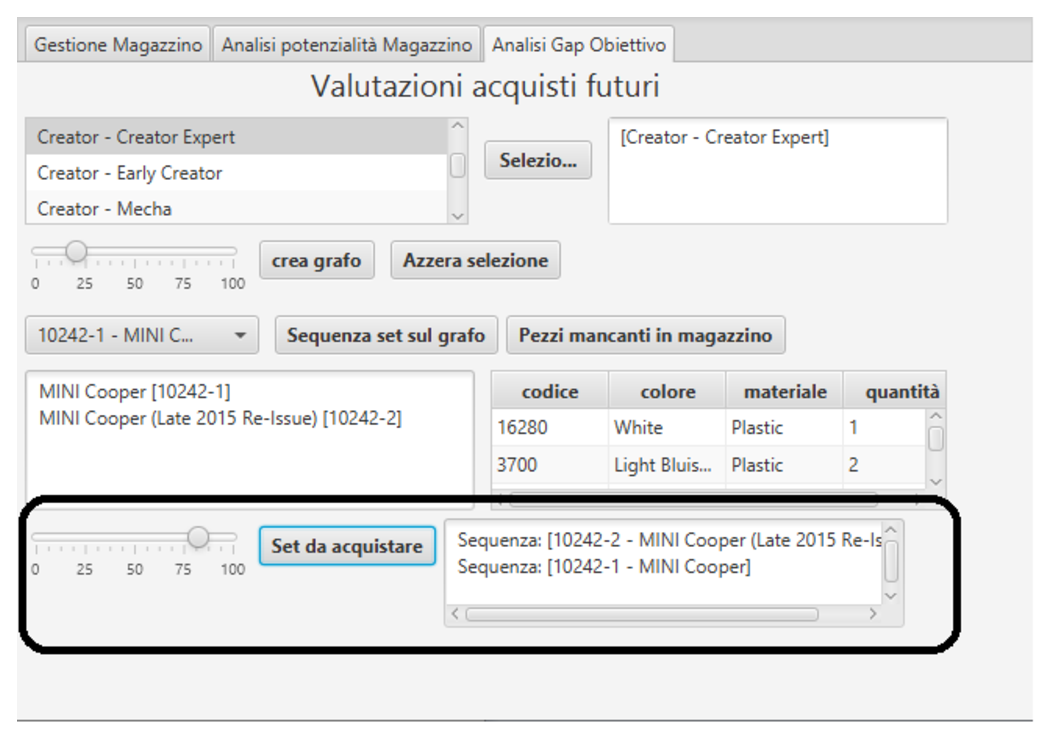
\includegraphics[scale=0.6]{interfaccia_grafica/gap.eps}
\end{figure}

\section {Video dimostrativo del software}

\url{https://youtu.be/JzkvN3o1dbM}